\documentclass{article}
\usepackage[utf8]{inputenc}
\usepackage[papersize={8.5in,11in},margin=0.8in]{geometry}
\usepackage{xcolor}
\usepackage{color, colortbl}
\usepackage{graphicx}
\usepackage{tikz}
\usepackage{amssymb}
\usepackage{multicol}
\definecolor{LightCyan}{rgb}{0.88,1,1}
\definecolor{LightRed}{rgb}{1,0.49,0.49}
\def\rectset{(-4,-2.5) rectangle (2,2)}
\def\circleone{(-1.9,0.5) circle (1.2cm)}
\def\circletwo{(-0.1,0.5) circle (1.2cm)}
\def\circlethree{(-1,-1) circle (1.2cm)}

\title{MATH 505 HW 4}
\author{John Caruthers}
\date\today

\begin{document}
\maketitle

\textbf{Section 2.1}

\begin{itemize}
    \item[Exp 2.] Recall that in Example 3, we found eight subsets of the set \{\emph{a}, \emph{b}, \emph{c}\}.
    
    (a) List all the subsets of \{\emph{a}, \emph{b}\}.\\
    {\color{blue} \{\emph{}\}, \{\emph{a}\}, \{\emph{b}\},\{\emph{a,b}\}}
    
    (b) List all the subsets of \{\emph{a}, \emph{b}, \emph{c}, \emph{d}\}.\\
    {\color{blue} \{\emph{}\}, \{\emph{a}\}, \{\emph{b}\},\{\emph{c}\},\{\emph{d}\},\{\emph{a,b}\},\{\emph{a,c}\},\{\emph{b,c}\},\{\emph{a,d}\},\{\emph{b,d}\},\{\emph{c,d}\},\{\emph{a,b,c}\},\{\emph{a,b,d}\},\{\emph{a,d,c}\},\{\emph{d,b,c}\},\{\emph{a,b,c,d}\}}
    
    (c) Make a conjecture about the number of subsets of a set with five elements.\\
    {\color{blue} 32.}
    
    (d) Check guess in (c) by listing all the subsets of \{\emph{a}, \emph{b}, \emph{c}, \emph{d}, \emph{e}\}.\\
    {\color{blue} \{\emph{}\}, \{\emph{a}\}, \{\emph{b}\},\{\emph{c}\},\{\emph{d}\},\{\emph{e}\},\{\emph{a,b}\},\{\emph{a,c}\},\{\emph{a,d}\},\{\emph{a,e}\},\{\emph{b,c}\},\{\emph{b,d}\},\{\emph{b,e}\},\{\emph{c,d}\},\{\emph{c,e}\},\{\emph{d,e}\},\{\emph{a,b,c}\},\{\emph{a,b,d}\},\\\{\emph{a,b,e}\},\{\emph{a,c,d}\},\{\emph{a,c,e}\},\{\emph{a,d,e}\},\{\emph{b,c,d}\},\{\emph{b,c,e}\},\{\emph{b,d,e}\},\{\emph{c,d,e}\},\{\emph{a,b,c,d}\},\{\emph{a,b,c,e}\},\{\emph{a,b,d,e}\},\{\emph{a,c,d,e}\},\\\{\emph{b,c,d,e}\},\{\emph{a,b,c,d,e}\}}
    
    (e) Make a conjecture about the number of subsets of a set with \emph{n} elements.\\
    {\color{blue} I assume that the number of subsets is $n^2$ with $n$ being the number of elements in the set.}
    
    \item[Exp 3.] A town board consists of six people: Al, Bo, Cy, Di, Ed, and Flo.  To be approved, a resolution must receive the votes of a majority (more than half) of the board members.  List all possible successful voting coalitions as subsets of the set of town board members.\\
    {\color{blue}  \{\emph{Al,Bo,Cy,Di}\},\{\emph{Al,Bo,Cy,Ed}\},\{\emph{Al,Bo,Cy,Flo}\},\{\emph{Al,Bo,Di,Ed}\},\{\emph{Al,Bo,Di,Flo}\},\{\emph{Al,Bo,Ed,Flo}\},\\\{\emph{Al,Cy,Di,Ed}\},\{\emph{Al,Cy,Di,Flo}\},\{\emph{Al,Cy,Ed,Flo}\},\{\emph{Al,Di,Ed,Flo}\},\{\emph{Bo,Cy,Di,Ed}\},\{\emph{Bo,Cy,Di,Flo}\},\\\{\emph{Bo,Cy,Ed,Flo}\},\{\emph{Bo,Di,Ed,Flo}\},\{\emph{Cy,Di,Ed,Flo}\},\{\emph{Al,Bo,Cy,Di,Ed}\},\{\emph{Al,Bo,Cy,Di,Flo}\},\{\emph{Al,Bo,Cy,Ed,Flo}\},\\\{\emph{Al,Bo,Di,Ed,Flo}\},\{\emph{Al,Cy,Di,Ed,Flo}\},\{\emph{Bo,Cy,Di,Ed,Flo}\},\{\emph{Al,Bo,Cy,Di,Ed,Flo}\}}
    
    \item[1.] Let $A = \{1, 2, 3, 4, 5\}$. Classify each of the following statements as true or false.
        \begin{multicols}{2}
        (a) $2 \in A.$ {\color{blue} T}
        
        (c) $0 \in A.$ {\color{blue} F}
        
        (e) $\oslash \subset A.$ {\color{blue} T}
        
        (g) $\{1,2,3\} \subseteq A.$ {\color{blue} T}
        
        (i) $4 \subset A.$ {\color{blue} F}
        
        \columnbreak
        (b) $\{2\} \in A.$ {\color{blue} F}
        
        (d) $\oslash \in A.$ {\color{blue} F}
        
        (f) $\{1,2,3\} \in A.$ {\color{blue} F}
        
        (h) $\{1,2,3\} \subset A.$ {\color{blue} T}
        
        (j) $\{1,2,3,4,5\} \subset A.$ {\color{blue} F}
        
        \end{multicols}
        
    \item[2.] Let $A = \{2,4,8\}$. In each of the following statements, fill in the blank with one of the symbols $\in, \notin, \subset,$ or $\not\subset$ in order to make the statement true.
        \begin{multicols}{2}
        (a) 0 \textcolor{blue}{$\notin$} $A$.
        
        (c) 2 \textcolor{blue}{$\in$} $A$.
        
        (e) $\{8\}$ \textcolor{blue}{$\subset$} $A$.
        
        (g) $\{2,4,6\}$ \textcolor{blue}{$\not\subset$} $A$.
        
        (i) $\oslash$ \textcolor{blue}{$\subset$} $A$.
        
        \columnbreak
        (b) $\{0\}$ \textcolor{blue}{$\not\subset$}  $A$.
        
        (d) 6 \textcolor{blue}{$\notin$} $A$.
        
        (f) $\{2,4\}$ \textcolor{blue}{$\subset$} $A$.
        
        (h) $\{2,4,8\}$ \textcolor{blue}{$\subseteq$} $A$.
        
        (j) $\{\oslash\}$ \textcolor{blue}{$\not\subset$} $A$.
        
        \end{multicols}
        
    \newpage
    \item[3.] Describe the set B in example 1 in the this section using the listing method.

    {\color{blue} $B = \{2,4,6,8\}$}
    
    \item[4.] Write the sets B and C of Example 1 in this section using set-builder notation.
    
    {\color{blue} $B = \{n|n $ is an even integer with $n > 0$ and $n < 10$\}}
    
    {\color{blue} $C = \{n|n$ is US President elected before 2003\}}
    
    \item[5.] Let $E = \{n|n$ is an integer and $n^2 < 10$\}. Describe $E$ using the listing method.
    
    {\color{blue} $E = \{-3, -2, -1, 0, 1, 2, 3\}$}
    
    \item[6.] Describe each of the following sets using the listing methods.
    
    (a) The set of all single-digit odd counting numbers\\
    \hspace*{0.6cm}{\color{blue}$S = \{1, 3, 5, 7, 9\}$}
    
    (b) The set of all living former U.S. presidents\\
    \hspace*{0.6cm}{\color{blue} $S = \{$Jimmy Carter, Bill Clinton, George W. Bush, Barack Obama, Donald Trump\}}
    
    (c) The set of all U.S. state capitals that were named for U.S. presidents\\
    \hspace*{0.6cm}{\color{blue} $S = $\{Lincoln NE, Jackson MS, Madison WI, Jefferson City MO\}}
    
    (d) The set of all square numbers less than 50\\
    \hspace*{0.6cm}{\color{blue} $S = $\{0, 1, 4, 9, 16, 25, 36, 49\}}
    
    (e) The set of all even counting numbers\\
    \hspace*{0.6cm}{\color{blue} $S = $\{2, 4, 6, 8, 10, 12, ...\}}
    
    \item[7.] Describe each of the sets in the previous exercise using set-builder notation.
    
    (a) {\color{blue} $S = \{x|x$ is odd counting number, $x <10\}$}
    
    (b) {\color{blue} $S = \{x|x$ is a living former US presidents$\}$}
    
    (c) {\color{blue} $S = \{x|x$ is state capitals named after U.S. Presidents$\}$}
    
    (d) {\color{blue} $S = \{x^2|x\in\mathbb{Z}, x^2 < 50\}$}
    
    (e) {\color{blue} $S = \{x|x\in\mathbb{Z}, x$ is even$\}$}
    
    \item[8.] Give a verbal description of each of the following sets:
    
    (a) $\{a, e, i, o, u, y\}$\\
    \hspace*{0.6cm}{\color{blue}Set containing all vowels.}
    
    (b) $\{1,2,3,4,5,6,7,8,9\}$\\
    \hspace*{0.6cm}{\color{blue}Set containing all natural numbers less than 10.}
    
    (c) \{Sunday, Monday, Tuesday, ..., Saturday\}\\
    \hspace*{0.6cm}{\color{blue}Set of all day names in a 7 day week.}
    
    (d) $\{..., -5, -3, -1, 1, 3, 5, ...\}$\\
    \hspace*{0.6cm}{\color{blue}Set of all integers.}
    
    (e) \{Mercury, Venus, Earth, Mars, Jupiter, Saturn, Uranus, Neptune, Pluto\}\\
    \hspace*{0.6cm}{\color{blue}Set of all planet names including Pluto.}
    
    \item[9.] Describe each of the following sets using the listing method:
    
    (a) $\{x|x$ is an odd counting number with one digit\}\\
    \hspace*{0.6cm}{\color{blue}$S = \{1, 3, 5, 7, 9\}$}
    
    (b) $\{x|x^2 = 9\}$\\
    \hspace*{0.6cm}{\color{blue}$S = \{-3, 3\}$}
    
    (c) $\{x|x$ is a two-digit counting number that looks the same upside down as right-side up\}\\
    \hspace*{0.6cm}{\color{blue}$S = \{11,69, 88, 96\}$}
    
    (d) $\{x|x$ is a state in the United States that begins with the letter A\}\\
    \hspace*{0.6cm}{\color{blue}$S = \{$Alaska, Arkansas, Alabama, Arizona$\}$}
    
    \item[11.] Which of the following represent equal sets?
    
    $A = \{1, 2, 3, 4, 5\}$
    
    $B = \{a, b, c, d, e\}$
    
    $C = \{1, 4, 2, 5, 3\}$
    
    $D = \{1, 1, 2, 3, 4, 4, 5, 5, 5\}$
    
    $E = \{x|x$ is a counting number less than 5\}
    
    {\color{blue}$A, C, D$ are all equal sets.}
    
    \item[12.] Which of the following represent equal sets?
    
    $A = \{\}$
    
    $B = \{\oslash\}$
    
    $C = \oslash$
    
    $D = 0$
    
    $E = \{0\}$
    
    {\color{blue}$A$ and $C$ are equal sets.}
    
    \item[15.] Let $U$ be the set of months of the year; let $A$ be the set of months that have exactly 30 days; let $B$ be the set of months that begin with the letter "J"; let $C$ be the months that contain the letter "R". Describe each of the following sets using the listing method.\\
    $U = \{$Jan, Feb, Mar, Apr, May, Jun, Jul, Aug, Sep, Oct, Nov, Dec$\}$\\
    $A = \{$Apr, Jun, Sep, Nov$\}$\\
    $B = \{$Jan, Jun, Jul$\}$\\
    $C = \{$Jan, Feb, Mar, Apr, Sep, Oct, Nov, Dec$\}$
    
    (a) $A \cup B$
    {\color{blue}$= \{$Jan, Apr, May, Jun, Jul, Sep, Nov$\}$}
    
    (b) $B \cap C$
    {\color{blue}$= \{$Jan$\}$}
    
    (c) $\overline C$
     {\color{blue}$= \{$May, Jun, Jul, Aug$\}$}
    
    (d) $B \cup \overline C$
    {\color{blue}$= \{$Jan, May, Jun, Jul, Aug$\}$}
    
    (e) $\overline B \cap C$
    {\color{blue}$= \{$Feb, Mar, Apr, Sep, Oct, Nov, Dec$\}$}
    
    \item[16.] Shade the portion of the Venn diagram below that illustrates each of the following sets:
    
    (a) $A \cup B$\\
    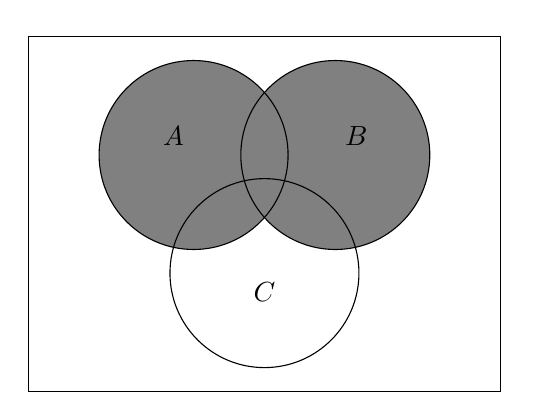
\begin{tikzpicture}
        \begin{scope}
    \clip \rectset;
        \end{scope}
        \begin{scope}
    \clip \circleone;
    \fill[gray] \circleone;
        \end{scope}
        \begin{scope}
    \clip \circletwo;
    \fill[gray] \circletwo;
        \end{scope}
        \begin{scope}
    \clip \circlethree;
        \end{scope}
    \draw \rectset node {};
    \draw \circleone node[text=black,above left] {$A$};
    \draw \circletwo node[text=black, above right] {$B$};
    \draw \circlethree node[text=black, below] {$C$};
    \end{tikzpicture}
    
    \newpage
    (b) $B \cap C$\\
    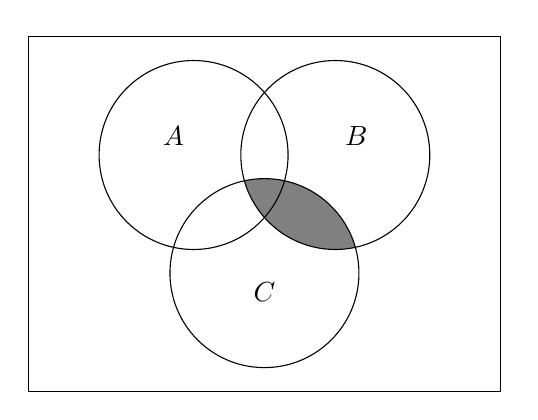
\begin{tikzpicture}
        \begin{scope}
    \clip \rectset;
        \end{scope}
        \begin{scope}
    \clip \circleone;
        \end{scope}
        \begin{scope}
    \clip \circletwo;
    \fill[gray] \circlethree;
        \end{scope}
        \begin{scope}
    \clip \circlethree;
        \end{scope}
    \draw \rectset node {};
    \draw \circleone node[text=black,above left] {$A$};
    \draw \circletwo node[text=black, above right] {$B$};
    \draw \circlethree node[text=black, below] {$C$};
    \end{tikzpicture}
    
    (c) $(A \cup C) \cap B$\\
    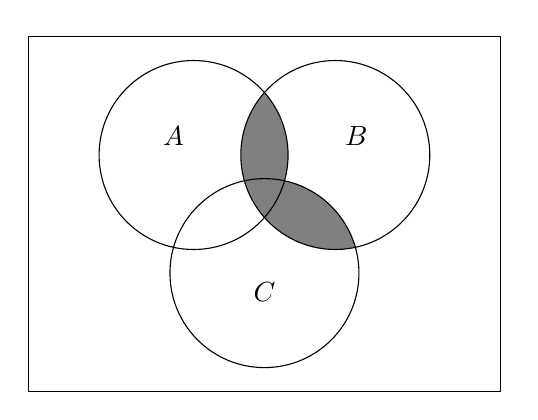
\begin{tikzpicture}
        \begin{scope}
    \clip \rectset;
        \end{scope}
        \begin{scope}
    \clip \circleone;
        \end{scope}
        \begin{scope}
    \clip \circletwo;
    \fill[gray] \circleone;
    \fill[gray] \circlethree;
        \end{scope}
        \begin{scope}
    \clip \circlethree;
        \end{scope}
    \draw \rectset node {};
    \draw \circleone node[text=black,above left] {$A$};
    \draw \circletwo node[text=black, above right] {$B$};
    \draw \circlethree node[text=black, below] {$C$};
    \end{tikzpicture}
    
    (d) $B \cup \overline C$\\
    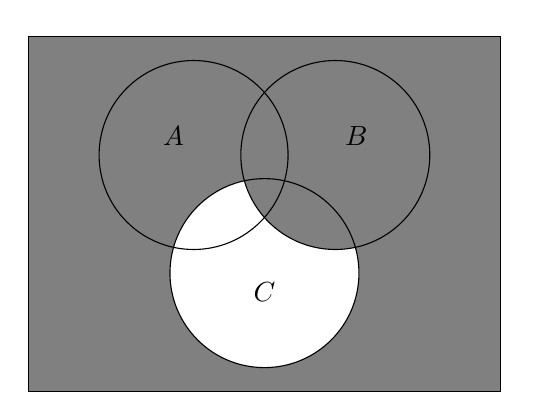
\begin{tikzpicture}
        \begin{scope}
    \clip \rectset;
    \fill[gray] \rectset;
        \end{scope}
        \begin{scope}
    \clip \circleone;
        \end{scope}
        \begin{scope}
    \clip \circletwo;
        \end{scope}
        \begin{scope}
    \clip \circlethree;
    \fill[white] \circlethree;
    \fill[gray] \circletwo;
        \end{scope}
    \draw \rectset node {};
    \draw \circleone node[text=black,above left] {$A$};
    \draw \circletwo node[text=black, above right] {$B$};
    \draw \circlethree node[text=black, below] {$C$};
    \end{tikzpicture}
    
    (e) $\overline B \cap C$\\
    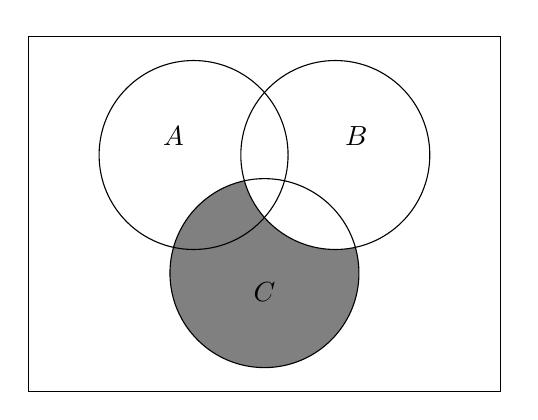
\begin{tikzpicture}
        \begin{scope}
    \clip \rectset;
        \end{scope}
        \begin{scope}
    \clip \circleone;
        \end{scope}
        \begin{scope}
    \clip \circletwo;
        \end{scope}
        \begin{scope}
    \clip \circlethree;
    \fill[gray] \circlethree;
    \fill[white] \circletwo;
        \end{scope}
    \draw \rectset node {};
    \draw \circleone node[text=black,above left] {$A$};
    \draw \circletwo node[text=black, above right] {$B$};
    \draw \circlethree node[text=black, below] {$C$};
    \end{tikzpicture}
    
    \newpage
    
    (f) $A \cap \overline B \cap C$\\
    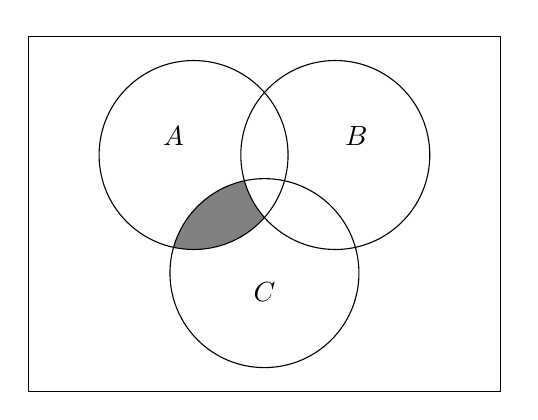
\begin{tikzpicture}
        \begin{scope}
    \clip \rectset;
        \end{scope}
        \begin{scope}
    \clip \circleone;
    \fill[gray] \circlethree;
        \end{scope}
        \begin{scope}
    \clip \circletwo;
    \fill[white] \circletwo;
        \end{scope}
        \begin{scope}
    \clip \circlethree;
        \end{scope}
    \draw \rectset node {};
    \draw \circleone node[text=black,above left] {$A$};
    \draw \circletwo node[text=black, above right] {$B$};
    \draw \circlethree node[text=black, below] {$C$};
    \end{tikzpicture}
    
    \item[17.] In each of the following Venn diagrams, describe the shaded region both verbally and in terms of unions, intersections, and complements of the sets $A, B,$ and $C$.
    
    (a)\\
    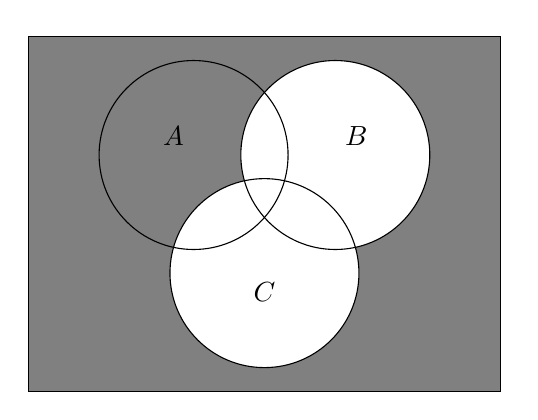
\begin{tikzpicture}
        \begin{scope}
    \clip \rectset;
    \fill[gray] \rectset;
        \end{scope}
        \begin{scope}
    \clip \circleone;
        \end{scope}
        \begin{scope}
    \clip \circletwo;
    \fill[white] \circletwo;
        \end{scope}
        \begin{scope}
    \clip \circlethree;
    \fill[white] \circlethree;
        \end{scope}
    \draw \rectset node {};
    \draw \circleone node[text=black,above left] {$A$};
    \draw \circletwo node[text=black, above right] {$B$};
    \draw \circlethree node[text=black, below] {$C$};
    \end{tikzpicture}
    
    {\color{blue} Verbal: Everything in the universal set except for C and B
    
    Symbol: $\overline{(B \cup C)}$}
    
    (b)\\
    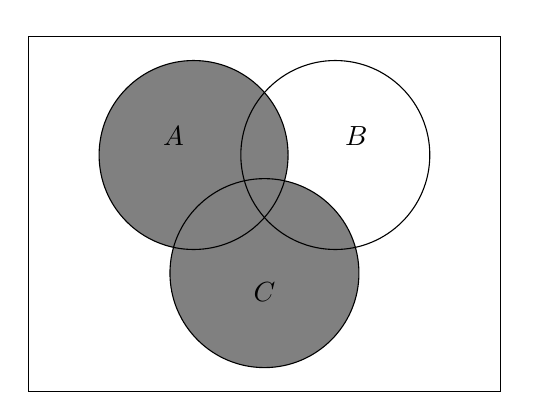
\begin{tikzpicture}
        \begin{scope}
    \clip \rectset;
        \end{scope}
        \begin{scope}
    \clip \circleone;
    \fill[gray] \circleone;
        \end{scope}
        \begin{scope}
    \clip \circletwo;
        \end{scope}
        \begin{scope}
    \clip \circlethree;
    \fill[gray] \circlethree;
        \end{scope}
    \draw \rectset node {};
    \draw \circleone node[text=black,above left] {$A$};
    \draw \circletwo node[text=black, above right] {$B$};
    \draw \circlethree node[text=black, below] {$C$};
    \end{tikzpicture}
    
    {\color{blue} Verbal: A and C
    
    Sybmol: $A \cup C$}
    
    \item[18.] Let $A = \{1, 2, 3, 4\}$.
    
    (a) List all subsets of $A$ that have four elements. How many are there?
    
    {\color{blue}There is one subset: $\{1, 2, 3, 4\}$ }
    
    (b) List all subsets of $A$ that have three elements. How many are there?
    
    {\color{blue}There are four subsets: $\{1, 2, 3\}, \{1, 2, 4\}, \{1, 3, 4\}, \{2, 3, 4\}$}
    
    (c) List all subsets of $A$ that have two elements. How many are there?
    
    {\color{blue} There are six subsets: $\{1, 2\}, \{1, 3\}, \{1, 4\}, \{2, 3\}, \{2, 4\}, \{3, 4\}$}
    
    \newpage
    
    (d) List all subsets of $A$ that have one elements. How many are there?
    
    {\color{blue} There are four subsets: $\{1\}, \{2\}, \{3\}, \{4\}$}
    
    (e) List all subsets of $A$ that have no elements. How many are there?
    
    {\color{blue} There is one null subset: $\{\}$}
    
    (f) How many subsets does $A$ have?
    
    {\color{blue} There are 16 total subsets.}
    
    \item[19.] In the Venn diagram below, sets $A, B,$ and $C$ are subsets of the universal subset $U$.  Label each of the following eight disjoint sets in the diagram below.  Mark the first set with a 1, the second with a 2, and so on.
    
    \begin{multicols}{2}
    
    (1) $A \cap B \cap C$
    
    (2) $\overline{A} \cap B \cap C$
    
    (3) $A \cap \overline{B} \cap C$
    
    (4) $A \cap B \cap \overline{C}$
    
    \columnbreak
    
    (5) $\overline{A} \cap \overline{B} \cap C$
    
    (6) $\overline{A} \cap B \cap \overline{C}$
    
    (7) $A \cap \overline{B} \cap \overline{C}$
    
    (8) $\overline{A} \cap \overline{B} \cap \overline{C}$
    
    \end{multicols}
    
    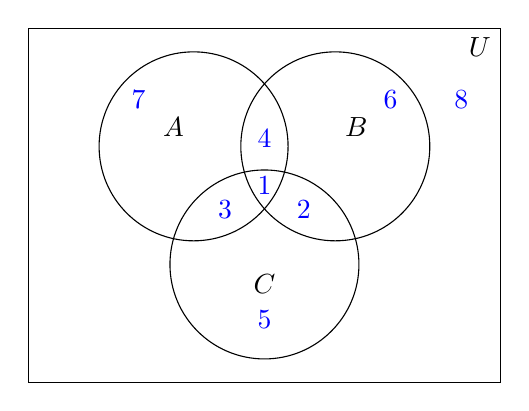
\begin{tikzpicture}
        \begin{scope}
    \clip \rectset;
        \end{scope}
        \begin{scope}
    \clip \circleone;
        \end{scope}
        \begin{scope}
    \clip \circletwo;
        \end{scope}
        \begin{scope}
    \clip \circlethree;
        \end{scope}
    \draw \rectset node[text=black, below left] {$U$};
    \draw \circleone node[text=black,above left] {$A$};
    \draw \circletwo node[text=black, above right] {$B$};
    \draw \circlethree node[text=black, below] {$C$};
    
    \node[blue] at (-1,0) {$1$};
    \node[blue] at (-0.5,-0.3) {$2$};
    \node[blue] at (-1.5,-0.3) {$3$};
    \node[blue] at (-1,0.6) {$4$};
    \node[blue] at (-1,-1.7) {$5$};
    \node[blue] at (0.6,1.1) {$6$};
    \node[blue] at (-2.6,1.1) {$7$};
    \node[blue] at (1.5,1.1) {$8$};
    
    \end{tikzpicture}
    
    \textbf{Section 2.2}
    
    \item[Exp 8.] Your younger brother is having difficulty understanding the reflexive, symmetric, and transitive properties of relations.  Write a paragraph explaining to him, using words rather than symbols, what each of these three properties means.  As an example, include an explanation of which properties the relation "is a brother of" satisfies on the set of all people. 
    
    {\color{blue} Imagine your sports team, Each person on the team is an athlete of that team, which is a reflexive relationship.  Each athlete is a teammate of the other athletes on the team, which is a symmetric relationship.  Now imagine that you lined up the athletes by 40m sprint speed.  The fastest athlete would be faster than the guy before him and so on down to the slowest athlete.  This is a transitive relationship.}
    
    {\color{blue} }
    
    \item[2.] Let $A = \{x, y, z\}$ and $B = \{1, 2, 3\}$. List the elements of each of the following Cartesian products.
    
    (a) $A \times B$ {\color{blue} = $\{(x,1), (x,2), (x,3), (y,1), (y,2), (y,3), (z,1), (z,2), (z,3)\}$}
    
    (b) $B \times A$ {\color{blue} = $\{(1,x), (1,y), (1,z), (2,x), (2,y), (2,z), (3,x), (3,y), (3,z)\}$}
    
    \item[3.] Determine the number of elements in the Cartesian product $A \times B$ if:
    
    (a) $A = \{2, 4, 6, 7\}$ and $B = \{1, 3, 4, 5, 6\}$ {\color{blue} $n(A \times B) = n(A) \times n(B) = 4\times5 = 20$} 
    
    (b) $A = \{1, 2, 3, 4, 5\}$ and $B = \{a, b, c, ..., z\}$ {\color{blue} $n(A \times B) = n(A) \times n(B) = 5 \times 26 = 130$} 
    
    \item[4.] If $A = \{1, 2, 3, 4\}, B = \{5, 6, 7\}$, and $C = \{8, 9\}$, determine the number of elements in each of the following Cartesian products:
    
    (a) $A \times B$ {\color{blue} 12}
    
    (b) $A \times C$ {\color{blue} 8}
    
    (c) $B \times C$ {\color{blue} 6}
    
    (d) $(A \times B) \times C$ {\color{blue} 24}
    
    \item[6.] Describe each of the following relations on the set $A = \{1, 2, 3\}$ as a subset of $A \times A$.\\
    {\color{blue} $A \times A = \{ (1,1),(1,2),(1,3),(2,1),(2,2),(2,3),(3,1),(3,2),(3,3)\}$}
    
    (a) is less than {\color{blue} This property is transitive and applies to this set}
    
    (b) is less than or equal to {\color{blue} This property applies to the set since $(1,1), (2,2), (3,3)$ are in the set.}
    
    (c) equals {\color{blue} This property applies to the set because $(1,1), (2,2), (3,3)$ are in the set.}
    
    (d) is not equal to {\color{blue} This property applies the set as well.}
    
    \item[10.] Determine whether each of the following relations is reflexive, symmetric, or transitive on the set of all people:
    
    (a) is younger than
    {\color{blue} transitive}
    
    (b) was born in the same city as {\color{blue} symmetric}
    
    (c) likes {\color{blue} symmetric (assuming the other people like them too), reflexive (if the person likes themselves) and transitive (in a friend group of people that all like each other)}
    
    (d) is a relative of {\color{blue} symmetric}
    
    \item[15.] Consider the set $A = \{$one, two, three, four, five, six, seven, eight, nine, ten\}. Identify the equivalence classes in each of the following relations on $A$.
    
    (a) begins with the same letter of the alphabet as
    
    {\color{blue} S = \{(one), (two, three, ten), (four, five), (six, seven), (eight), (nine)\}}
    
    (b) has the same number of letters as
    
    {\color{blue} S = \{(one, two, six, ten), (four, five, nine), (three, seven, eight)\}}
    
    (c) has the same remainder when divided by three as
    
    {\color{blue} S = \{(three, six, nine), (one, four, seven, ten), (two, five, eight)\}}
    
\end{itemize}

\end{document}
